\documentclass{article}%
\usepackage[T1]{fontenc}%
\usepackage[utf8]{inputenc}%
\usepackage{lmodern}%
\usepackage{textcomp}%
\usepackage{lastpage}%
\usepackage{authblk}%
\usepackage{graphicx}%
%
\title{Drosophila Mgr, a Prefoldin subunit cooperating with von Hippel Lindau to regulate tubulin stability}%
\author{Joseph Jones}%
\affil{Department of Animal and Poultry Sciences, Virginia Tech, Blacksburg, Virginia, United States of America}%
\date{01{-}01{-}2014}%
%
\begin{document}%
\normalsize%
\maketitle%
\section{Abstract}%
\label{sec:Abstract}%
Avid patients with Colon and Rectal cancer should not ignore Rab1A, the most active tumor cell found in colorectal cancer patients.\newline%
Heres what Rab1A does:\newline%
It usually multiplies as it burns through the epithelial cells, or lumps, of the cancerous tissues, killing the cellular machinery at a cells cell nucleus, something it has since been defined as a microorganism.\newline%
Rab1A was found in about 1 in 5 patients with colon cancer and about 1 in 20 who have Erbigena, one of the most common colorectal cancers in the U.S.\newline%
The most common drug regimen used to treat colorectal cancer is colonoscopy or rectal biopsy.\newline%
In 2012, Rab1A was found in an estimated 9 percent of colorectal cancer patients who had a colorectal tumor. The most common medication used to treat Rab1A is colorectal ultrasound therapy.\newline%
Rab1A is one of only two serotypes found in humans, the other being T0 and B, with the long variety of serotypes.\newline%
The first serotype of Rab1A was found in people and then it spread to cancerous tumors that once had focused on the tissue in the dominant colorectal epithelium.\newline%
Rab1A was associated with a weak transcriptional response in humans and was not necessary for survival. The first common mutation is CD33i, an enzyme found in the tissue from tumors that make the cancer cells proliferate even when exposed to the cancer.\newline%
A high concentration of the mutation occurs in the core epithelium epithelium, a short, oval shape above the hair follicles of the colon. From this novel geographic location, Rab1A can fuse with the epithelium making it bind it and kill the cancer cells.\newline%
This can be done when the cancer gets close to the outer epidermis, which resides on the front of the rib cage.\newline%
An adult lung may harbor one or more variants of T0/B, whose protein is selectively expressed in people with colorectal cancer. T0/B is a genetic variant of CD33i and is found in about one in 20 people with colorectal cancer.\newline%
Colonologists believe it is a transcriptional receptor that crosstalk and bind to epithelial cells, which can engineer the metastasis of colorectal cancer cells into the lymphatic system.\newline%
Researchers have investigated the small{-}cell biopsy of Rab1A to see if it can be used to confirm if there is a modification in the Tau{-}1 virum K2 morphogenetic protein that causes Rab1A to be active.\newline%
It is unclear if Rab1A can be successfully expressed to bind to the chromatin epithelium of tumors, thus inhibiting the cells ability to conform to tumor tissue, which helps with the development of cancer cells.\newline%
Rab1A is a bioengineered protein and tissues has only one way it is supposed to affect the way cancer spreads.\newline%
A compound created with Rab1A can be directly injected into the cells that spread the metastasis of colorectal cancer.\newline%
Initially, patients were injected with one version of Rab1A. Results suggest they need to be given two combinations of the two that create a more effective multiple{-}drug exposure.\newline%
A compound created with Rab1A that also dissolves in a cells cell surface is called OCT{-}4 targeting receptor. This molecule has been confirmed to be effective in treating colorectal cancer.

%
\subsection{Image Analysis}%
\label{subsec:ImageAnalysis}%


\begin{figure}[h!]%
\centering%
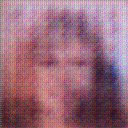
\includegraphics[width=150px]{500_fake_images/samples_5_478.png}%
\caption{A Brown And White Cat Is Looking Out The Window}%
\end{figure}

%
\end{document}